\documentclass[11pt,a4paper]{article}

\usepackage{polski}
%kodowanie widnows
%\usepackage[cp1250]{inputenc} 
%kodowanie linux
\usepackage[utf8]{inputenc}


%\usepackage[T1]{fontenc}
\usepackage{indentfirst}
\usepackage{wrapfig}    % for wrapping figures, tables

\frenchspacing

\usepackage{amssymb}
%\usepackage{bm}
\usepackage{gensymb}
%\usepackage{hepnames}
\usepackage{epsfig}
\usepackage{graphics}
\usepackage[shortlabels]{enumitem}
%\usepackage{xspace}
%\xspaceaddexceptions{[]\{\}}

%
%
%fixpagesize
\pagestyle{empty}
\addtolength{\textwidth}{6cm}
\addtolength{\textheight}{4cm}
\addtolength{\evensidemargin}{-3cm}
\addtolength{\oddsidemargin}{-3cm}
\addtolength{\topmargin}{-2cm}
\parindent=0cm


%
%
%small distance in list/item/enum for enumitem package
\setlist[itemize,enumerate]{topsep=0em}
\setlist{noitemsep}

%print zadanie #
\newcounter{zadanie}\newcommand{\zadanie}[1][]{\addtocounter{zadanie}{1} ~\\  {\bf \emph{Zadanie \arabic{zadanie} #1 }} \\}
\newcounter{zaddom}\newcommand{\zaddom}[1][]{\addtocounter{zaddom}{1} ~\\  {\bf \emph{Zadanie domowe \arabic{zaddom} #1 }} \\}
%\renewcommand{\zadanie}[1][]{\pagebreak  ~\\  {\bf \emph{Zadanie }} \\} \addtolength{\topmargin}{-2cm}


%%%%%%%%%%%%%%%%%%%%%%%%%%%%%%%%%%%%%%%%%%%%%%%%%%%%%%
\begin{document}           % End of preamble and beginning of text.
\vspace*{-1.8cm}

\begin{centering}
\bf{\Large{Termodynamika z elementami fizyki statystycznej}}\\
Ćwiczenia 3 \\[1mm]
ciśnienie, pływanie, równanie stanu, gaz doskonały \\
\end{centering}

\zadanie
Zależność objętości od ciśnienia dla pewnej substancji dana jest empirycznym wzorem $V(p) = V_0(1 + a\cdot p)^{-\alpha}$.
Wykazać, że w takim przypadku współczynnik ściśliwości $\kappa=-1/V(\partial V(p,T)/\partial p)_T$ spełnia relację: $1/\kappa=1/\kappa_0+c\cdot p$.
Wyznaczyć stałe $\kappa_0$ i $c$ przez $a$ i $\alpha$.

\zadanie
Okręt podwodny o stalowym kadłubie i masie m = $1000\textrm{t}$ jest zanurzony na głębokości peryskopowej tak, że siła wyporu jest dokładnie równa ciężarowi okrętu (pływalność zerowa). Temperatura wody wynosi przy tym 10\degree C. O ile trzeba zmienić balast okrętu, żeby utrzymać zerową pływalność po wpłynięciu na wodę o temperaturze 20\degree C? Współczynnik rozszerzalności objętościowej wody w tym zakresie temperatur wynosi $\gamma_w = 1.5\,10^{-4} K^{-1}$, zaś współczynnik rozszerzalności liniowej stali $\alpha_s = 1.2\,10^{-5} K^{-1}$. Ściśliwość wody i stali można zaniedbać.

%\vfill

\zadanie
Dla gazu doskonałego znajdź współczynniki:
\begin{itemize}
\item[1.] rozszerzalności objętościowej,
\item[2.] ściśliwości izotermicznej,
\item[3.] temperaturowej zmiany ciśnienia.
\end{itemize}
\phantom{.} \\
%\end{minipage}
\zadanie
W pionowym, znajdującym się w polu grawitacyjnym, zamkniętym cylindrze znajduje się gaz doskonały oraz dzielący naczynie masywny tłok, który może przemieszczać się bez tarcia. Z obu stron tłoka znajdują się jednakowe liczby cząstek gazu doskonałego. W temperaturze $T_0$, jednakowej w całym cylindrze, objętość górnej części jest $m$ razy większa niż objętość części dolnej. Jaki będzie stosunek tych objętości, jeśli temperatura wzrośnie do wartości $T_1$? Zaniedbać zmienność ciśnienia gazu z wysokością (tj. założyć, że w każdej z części cylindra ciśnienie jest stałe).

\zadanie
Wykazać, że dla gazu doskonałego zachodzi: $p = p_0 (1 + \frac{1}{273.15} T[\degree \textrm{C}])$ przy $V = \textrm{const}$,
oraz $V = V_0 (1+ \frac{1}{273.15}  T[\degree \textrm{C}])$ przy $p=\textrm{const}$, gdzie $p_0 =p(0\degree \textrm{C})$ i $V_0 =V(0\degree \textrm{C})$.

\vfill

\begin{minipage}{0.75\textwidth}
\zadanie
„Nurek” szklany ma kształt walca zamkniętego od góry i otwartego od dołu i pływa po powierzchni wody, nad którą panuje ciśnienie $p_0 = 1\,\textrm{bar}$ w taki sposób, że $h_1 = 2\textrm{mm}$ wystaje nad powierzchnię. Wewnątrz nurka jest powietrze, którego słupek ma wysokość $h_2 = 2\,\textrm{cm}$.
Jakie powinno być ciśnienie $p_0$ nad powierzchnią wody, aby nurek zatonął? Powietrze traktujemy jako gaz doskonały, jego masę zaniedbujemy. Grubość ścianek naczynia zaniedbujemy. Temperatura wody jest taka sama jak temperatura otoczenia.
%\begin{itemize}
%\%item[1.] rozszerzalności objętościowej,
%\item[2.] ściśliwości izotermicznej,
%\item[3.] temperaturowej zmiany ciśnienia.
%\end{itemize}
\phantom{.} \\
\end{minipage}
\begin{minipage}{0.25\textwidth}
\begin{center}

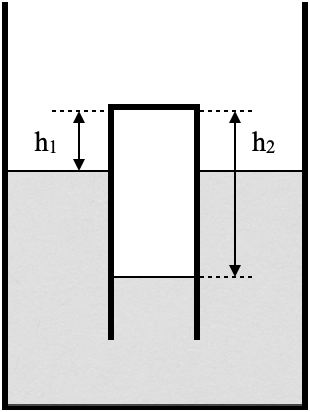
\includegraphics[width=0.85\textwidth]{zadanie8.png}
\end{center}
\end{minipage}

\begin{minipage}{0.65\textwidth}
    \zadanie
    Prostopadłościenny blok o wymiarach $a\times b\times c$ i gęstości $\rho_b$ zanurzono w wodzie o gęstości $\rho_w$ tak, 
    że jedna z jego ścianek była równoległa do tafli wody, a następnie odchylono od pionu o kąt $\alpha$ wokół osi równoległej
    do boku $c$. Bok $c$ jest dużo dłuższy od boków $a$ i $b$. Obliczyć wypadkowy moment 
    sił działający na blok i przedyskutować stabilność bloku ze względu na wychylenia. 
    %Kulka znajduje się w stanie równowagi pomiędzy dwoma cieczami (rysunek A) o~gęstościach $\rho_1 = 1.0\textrm{g}/\textrm{cm}^3$ i~$\rho_2 = 0.8\textrm{g}/\textrm{cm}^3$. Objętość zanurzona w cieczy ``1'' jest dwa razy większa niż objętość zanurzona w cieczy ``2''. Oblicz gęstość kulki.
    \end{minipage}
    \begin{minipage}{0.35\textwidth}
    \begin{center}
    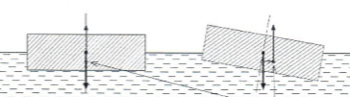
\includegraphics[width=1.0\textwidth]{plywanie3.png}
    \end{center}
\end{minipage}


%%%%%%%%%%%%%%%%%%%%%%%%%%%%%%%%%%%%%%%%%%%%%%%%%%%%%%
\newpage
%%%%%%%%%%%%%%%%%%%%%%%%%%%%%%%%%%%%%%%%%%%%%%%%%%%%%%

\zaddom
Walec o promieniu r i wysokości h zanurzono w wodzie. Nad powierzchnię wystaje 20\% wysokości walca. Jeżeli zanurzymy walec dodatkowo na niewielką głębokość $\Delta h$, a następnie puścimy swobodnie, to zacznie on drgać. Jaki to rodzaj ruchu? Jeśli jest to ruch periodyczny, to znajdź jego okres drgań $T$. Gęstość wody $\rho_w$ przyjmij jako znaną. Zaniedbaj opory związane z ruchem w ośrodku lepkim.\\
{\em Odpowiedź:} Walec będzie wykonywał drgania harmoniczne o okresie $T = 2\pi \sqrt{\frac{8h}{10g}}$.

\zaddom
Szklana butelka o pojemności $1\textrm\,{l}$ została napełniona do 95\% objętości olejem i szczelnie zakorkowana. Ciśnienie powietrza miało przy tym wartość normalną, a temperatura wynosiła 20\degree C. Następnie podgrzano butelkę o $\Delta T = 30\degree\textrm{C}$. Oblicz ciśnienie powietrza w podgrzanej butelce. Współczynnik rozszerzalności objętościowej oleju wynosi $\gamma = 8.5\,10^{-4} \textrm{K}^{-1}$, zaś współczynnik rozszerzalności liniowej szkła $\alpha  = 7.0\,10^{-6} \textrm{K}^{-1}$. Powietrze traktujemy jak gaz doskonały.\\
{\em Odpowiedź:} Dla początkowej ciśnienia $p_0 = 1013\,\textrm{hPa}$, ciśnienie po podgrzaniu będzie wynosić $2115\,\textrm{hPa}$.

\zaddom
Pustą i szczelną puszkę z dziurką w dnie zanurzono w wodzie, dziurką do dołu. Na jaką głębokość (liczoną od powierzchni wody do dna puszki) należy wepchnąć puszkę, aby już nie wypłynęła? Przyjmij, że: temperatura powietrza i wody jest stała, powietrze stosuje się do praw gazu doskonałego, a jego masę zaniedbujemy. Gęstość wody wynosi $\rho_w = 1.0\,\textrm{g/cm}^3$, masa puszki $m = 50\,\textrm{g}$, wymiary wewnętrzne puszki: średnica $d = 5\,\textrm{cm}$, wysokość $h = 20\textrm{cm}$.\\
{\em Odpowiedź:} $\frac{p_0(\rho_w V-m)}{mg\rho_w} - \frac{m}{\rho_wS} + h$,
gdzie $V = \pi\,d^2\,h/4$ jest objętością puszki, $S$ powierzchnią denka, a $p_0$ ciśnieniem atmosferycznym.

\end{document}

%%%%%%%%%%%%%%%%%%%%%%%%%%%%%%%%%%%%%%%%%%%%%%%%%%%%%%
\begin{minipage}{0.75\textwidth}
    \zaddom  
    Dwa baloniki o objętości $V_1$ i $V_2$ wypełnione powietrzem o ciśnieniu atmosferycznym połączono linką o długości L,
    a następnie zanurzono pod wodę przeciągając linę przez blok znajdujący się na głębokości $H$ (rysunek). Regulując
    odpowiednio wzajemne położenie baloników udało się doprowadzić do stanu, w którym żaden z nich nie wypływa ani się
    nie zanurza. Wyznaczyć różnicę zanurzeń $h$. Masy baloników, powietrza i linki pomijamy. Temperatura wody jest stała
    i równa temperaturze powietrza, które traktujemy jak gaz doskonały.\\
    
    \end{minipage}
    \begin{minipage}{0.25\textwidth}
    \begin{center}
    
    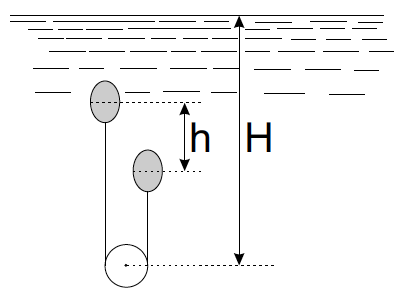
\includegraphics[width=0.85\textwidth]{baloniki.png}\\
    \end{center}
    \end{minipage}
%%%%%%%%%%%%%%%%%%%%%%%%%%%%%%%%%%%%%%%%%%%%%%%%%%%%%%    

